\documentclass{article}
\usepackage[utf8]{inputenc}
\usepackage[T1]{fontenc}
\usepackage{lmodern}
\usepackage[frenchb]{babel}
\usepackage{graphicx}
\usepackage[left=2cm,right=2cm,top=2cm,bottom=2cm]{geometry}
\usepackage{subcaption}

\title{Traitement des données Audio-Visuelle\\Projet}
\author{Victor Drouin Viallard}

\begin{document}

\maketitle
\clearpage
\tableofcontents
\clearpage

\section{TP1 - Espaces de représentation des couleurs}
\paragraph{}
Le but de ce TP est d'étudier les différentes façon de représenter les images couleurs, de les projeter dans des bases adaptées, et de les réduire à des espaces plus restreints.
\subsection{Exercice 1 - Corrélations et contrastes}
\paragraph{Corrélation des espaces RVB}
Ce premier exercice propose, sur une image particulière donnée, d'observer les corrélations existantes entre les différentes composantes colorimétriques. En effet, après calcul on obtient les coefficients de corrélation suivants entre les différentes couleurs~:
\begin{itemize}
    \item Rouge/Vert~: 0.9861
    \item Rouge/Bleu~: 0.9690
    \item Vert/Bleu~: 0.9918
\end{itemize}
Ce qui montre une très force corrélation entre les couleurs, tout particulièrement entre le vert et le bleu.

\paragraph{Non corrélation locale}
En outre, comme le suggère le sujet, on observe la disparition de l'arbre central de l'image sur sa composante bleu (figure~\ref{disparition_arbre}). Cela signifie que sur cette partie de l'image la corrélation entre la composante bleu et les autres composantes est assez faible.
\begin{figure}[ht]
    \centering
    \begin{subfigure}[c]{0.45\linewidth}
    	\centering
    	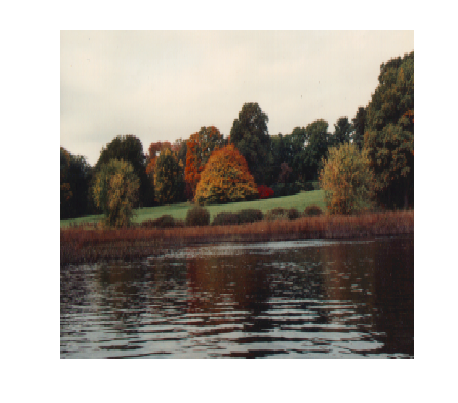
\includegraphics[width=\linewidth]{images/1/1-1-autumn_rgb.png}
    	\subcaption{Image originale}
    \end{subfigure}
    \hfill
    \begin{subfigure}[c]{0.45\linewidth}
    	\centering
    	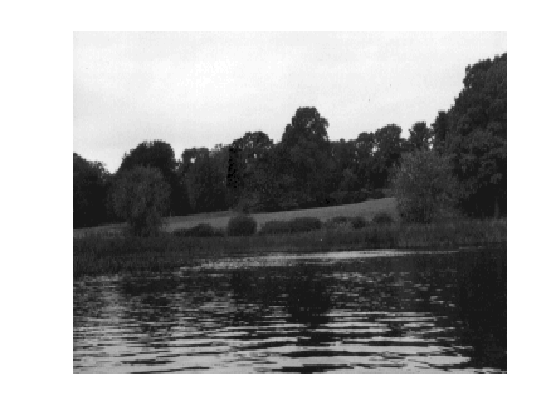
\includegraphics[width=\linewidth]{images/1/1-1-autumn_b.png}
    	\subcaption{Composante bleu}
    \end{subfigure}
    \caption{Disparition de l'arbre sur la composante bleu}
    \label{disparition_arbre}
    \label{truc}
\end{figure}
Si on choisit de calculer la corrélation entre les trois canaux dans cette zone de l'image, on observe en effet des valeurs différentes de celles précédentes car la corrélation entre le rouge et le bleu diminue fortement :
\begin{itemize}
    \item Rouge/Vert~: 0.8079
    \item Rouge/Bleu~: 0.1979
    \item Vert/Bleu~: 0.6671
\end{itemize}

d'où la disparition.

\paragraph{Contraste}
Le calcul de la variance des différentes composantes puis du contraste de l'image permet d'observer son faible niveau. Il est de : 0.3795 et se répartit comme suit entre les couleurs :
\begin{itemize}
    \item Rouge~: 0.3358
    \item Vert~: 0.3462
    \item Bleu~: 0.3179
\end{itemize}
Cette répartition uniforme est attendue du fait de la corrélation fortes entre les couleurs.

\paragraph{Transformation d'une image couleur en image noir et blanc}
Pour finir l'appel du script \emph{exercice\_2.m} sur l'image \emph{gantrycrane.png} permet, comme le laisse entendre le sujet, d'observer pourquoi le procédé de transformation d'une image couleur en image noir et blanc ne peut se faire par simple réduction à un canal choisi arbitrairement (figure~\ref{transmission_canal_bleu}). En effet, une image dont le contraste est, par exemple, dû à sa composante rouge ne pourra être transformée en noir et blanc en ne conservant que sa composante bleu sans quoi elle paraîtrait unie.
\begin{figure}[ht]
    \begin{center}
        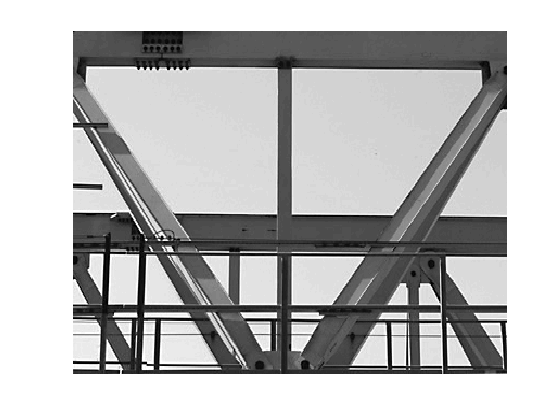
\includegraphics[width=0.6\linewidth]{images/1/1-1-gantrycrane_b.png}
        \caption{Transformation en noir et blanc par conservation du canal bleu}
        \label{transmission_canal_bleu}
    \end{center}
\end{figure}

\subsection{Exercice 2 - Analyse en composantes principales}
\paragraph{ACP}
Pour faire face au problème ennoncé plus haut qui est celui de la réduction d'un jeu de données par projection dans un espace de dimmension inférieur, l'idée la plus intéressante consiste à effectuer une analyse en composantes principales de l'objet. Celle-ci revient à trouver une base orthonormée de l'espace de départ pour laquelle la première composante représente la direction de plus grande variance, etc. En effectuant cette ACP sur la seconde image on observe la répartition des coefficiants selon les trois composantes (figure~\ref{acp_gantrycrane}).
\begin{figure}[ht]
    \centering
    \begin{subfigure}[c]{0.32\linewidth}
    	\centering
    	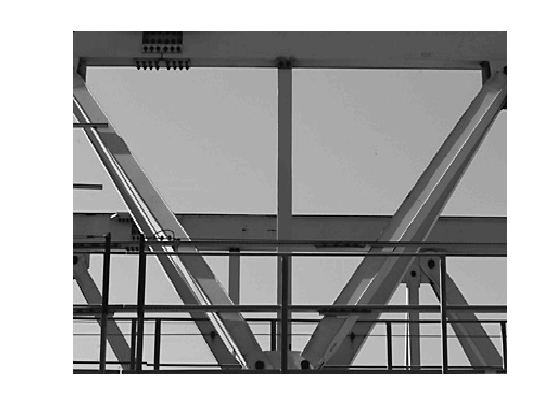
\includegraphics[width=\linewidth]{images/1/1-2-gantrycrane_c1.png}
    \end{subfigure}
    \hfill
    \begin{subfigure}[c]{0.32\linewidth}
    	\centering
    	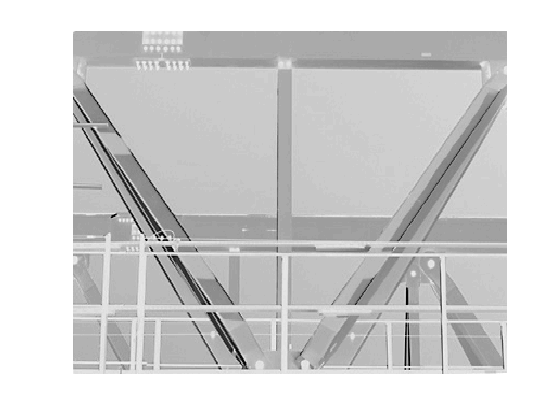
\includegraphics[width=\linewidth]{images/1/1-2-gantrycrane_c2.png}
    \end{subfigure}
    \hfill
    \begin{subfigure}[c]{0.32\linewidth}
    	\centering
    	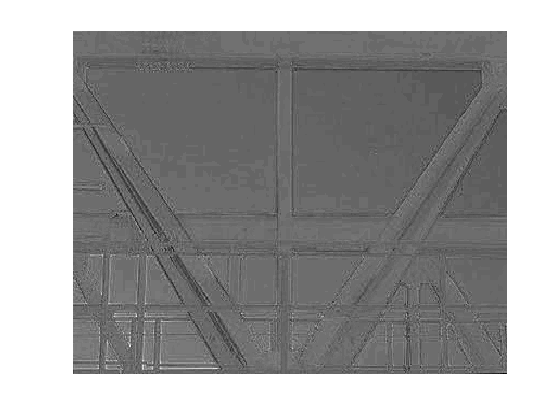
\includegraphics[width=\linewidth]{images/1/1-2-gantrycrane_c3.png}
    \end{subfigure}
    \caption{Résultat de l'analyse en composantes principales}
    \label{acp_gantrycrane}
\end{figure}
On voit alors que la première composante principale contient une information très proche de celle de l'image originale : c'est celle-ci qu'il faudrait transmettre pour une télévision en noir est blanc.
\paragraph{Conservation du constraste}
Pour la première image on réalise la même opération pour s'appercevoir alors que le la proportion de contraste est presque intégralement dûe à la première composante :
\begin{itemize}
	\item c1~: 0.9883
	\item c2~: 0.0103
	\item c3~: 0.0013
\end{itemize}
Cela est bien évidemment dû à la très forte corrélation entre les trois canaux de couleur. Enfin on remarque que le contraste se conserve entre les deux décompositions : cela est bien sûr le cas car le calcum du contraste est général au jeu de donnée et parfaitement indépendant de la base orthonormale dans laquelle elles sont exprimées.

\subsection{Exercice 3 - Combinaison des canaux RVB}
\paragraph{L'inconvénient de l'ACP}
Cette méthode de projection pour garder un maximum de contraste est la plus efficace mais extrêment coûteuse car nécessite pour chaque image de calculer et d'inverser la matrice de variance / covariance. La méthode retenue pour transmettre une image noir et blanc depuis une image en couleur a donc été d'effectuer une combinaison linéaire des trois canaux. On peut chosir plusieurs combinaisons linéaire différentes. Le sujet nous suggère de comparer celle uniforme et celle utilisée par la méthode \emph{rgb2gray} de Matlab (figure~\ref{combinaisons_canaux}).
\begin{figure}[ht]
    \centering
    \begin{subfigure}[c]{0.45\linewidth}
    	\centering
    	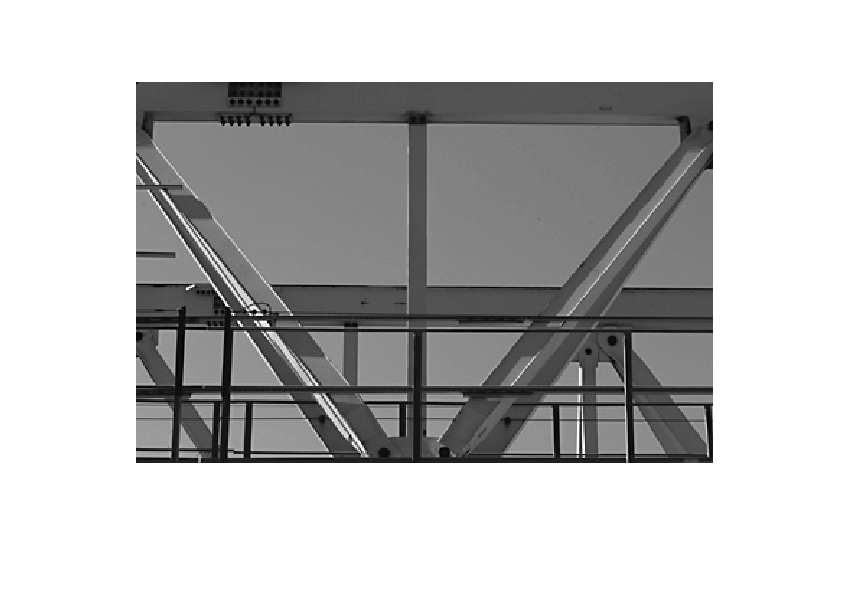
\includegraphics[width=\linewidth]{images/1/1-3-uniform.png}
    	\subcaption{Combinaison uniforme}
    \end{subfigure}
    \hfill
    \begin{subfigure}[c]{0.45\linewidth}
    	\centering
    	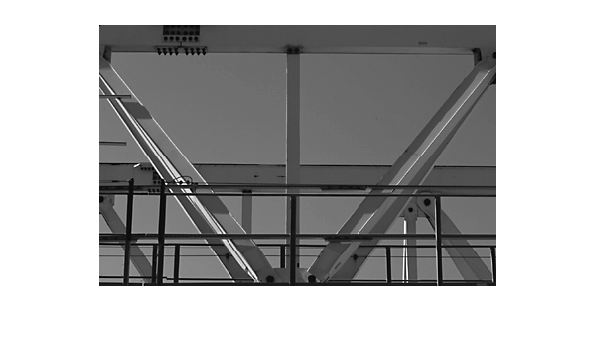
\includegraphics[width=\linewidth]{images/1/1-3-rgb2gray.png}
    	\subcaption{Combinaison par \emph{rgb2gray}}
    \end{subfigure}
    \caption{Transformation en noir et blanc par combinaisons linéaires des canaux de couleur}
    \label{combinaisons_canaux}
\end{figure}
Parmi toutes ces images en noir est blanc, c'est l'image issue du canal bleu qui paraît avoir le meilleur contraste mais cela est particulier et dû au fait que :
\begin{itemize}
	\item le bleu est effectivement un facteur de contraste de l'image
	\item l'ACP produisant des valeurs de coefficient négatives, l'affichage de la composante principale est biaisé
	\item la fonction d'affichage de matlab \emph{imshow} étale le spectre de l'image affichée ce qui peut conduire à un affichage qui paraît plus contrasté dans ce cas particulier
\end{itemize}
\section{TP2 - Eigenfaces}
Le but de ce TP est d'utiliser l'ACP pour établir une base de conaissance capable de restaurer une image dégradée à partir de sa projection dans cette base.
\subsection{Exercice 1 - Analyse en composantes principales}
Ce premier exercice ne présente pas de difficulté particulière mais permet de bien se rendre compte  du résultat de l'ACP sur un tel ensemble de données (figure~\ref{acp_faces}). On oberve en effet, sans doute car il y a des individus différents d'une photo à l'autre, que la première composante principale ne ressemble plus vraiment à un visage.
\begin{figure}[ht]
    \begin{center}
        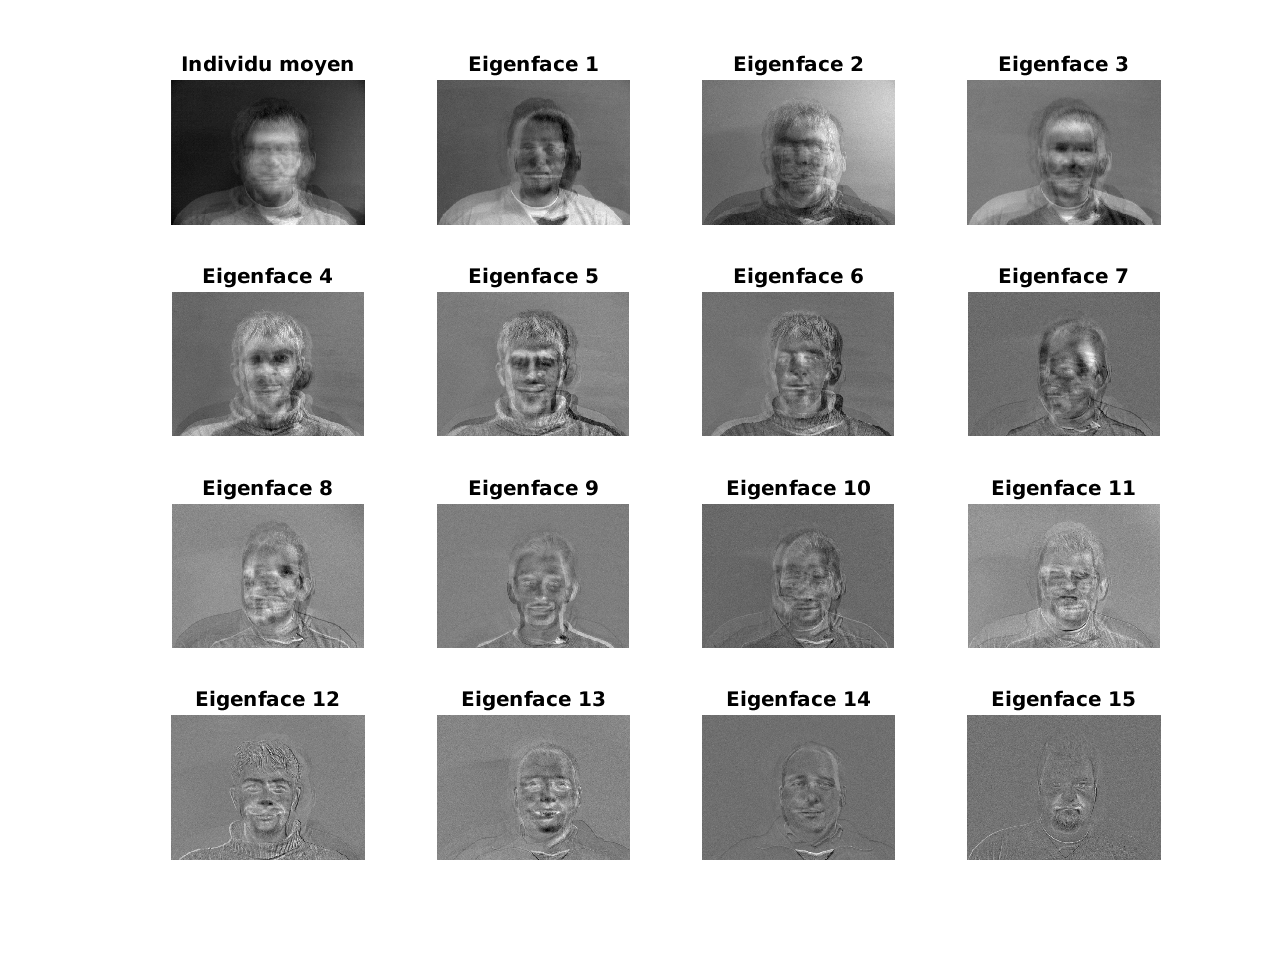
\includegraphics[width=0.9\linewidth]{images/2/2_1_res.png}
        \caption{Analyse en composantes principales des visages}
        \label{acp_faces}
    \end{center}
\end{figure}

\subsection{Exercice 2 - Projection des images sur les eigenfaces}
\paragraph{Différences selon l'individu et les images}
Dans cette exercice on nous propose d'exprimer les images des sujets dans la nouvelle base (celle composée des eigenfaces), puis de ne conserver qu'un certain nombre de composantes (projections selon les composantes de plus petit ordre) pour établir différentes "compressions" et les comparer. Par exemple en choisissant de ne conserver que 6 eigenfaces (sur 15) en plus de la valeur de l'infividu moyen, on obtient le résultat figure~\ref{proj_faces}.
\begin{figure}[ht]
    \begin{center}
        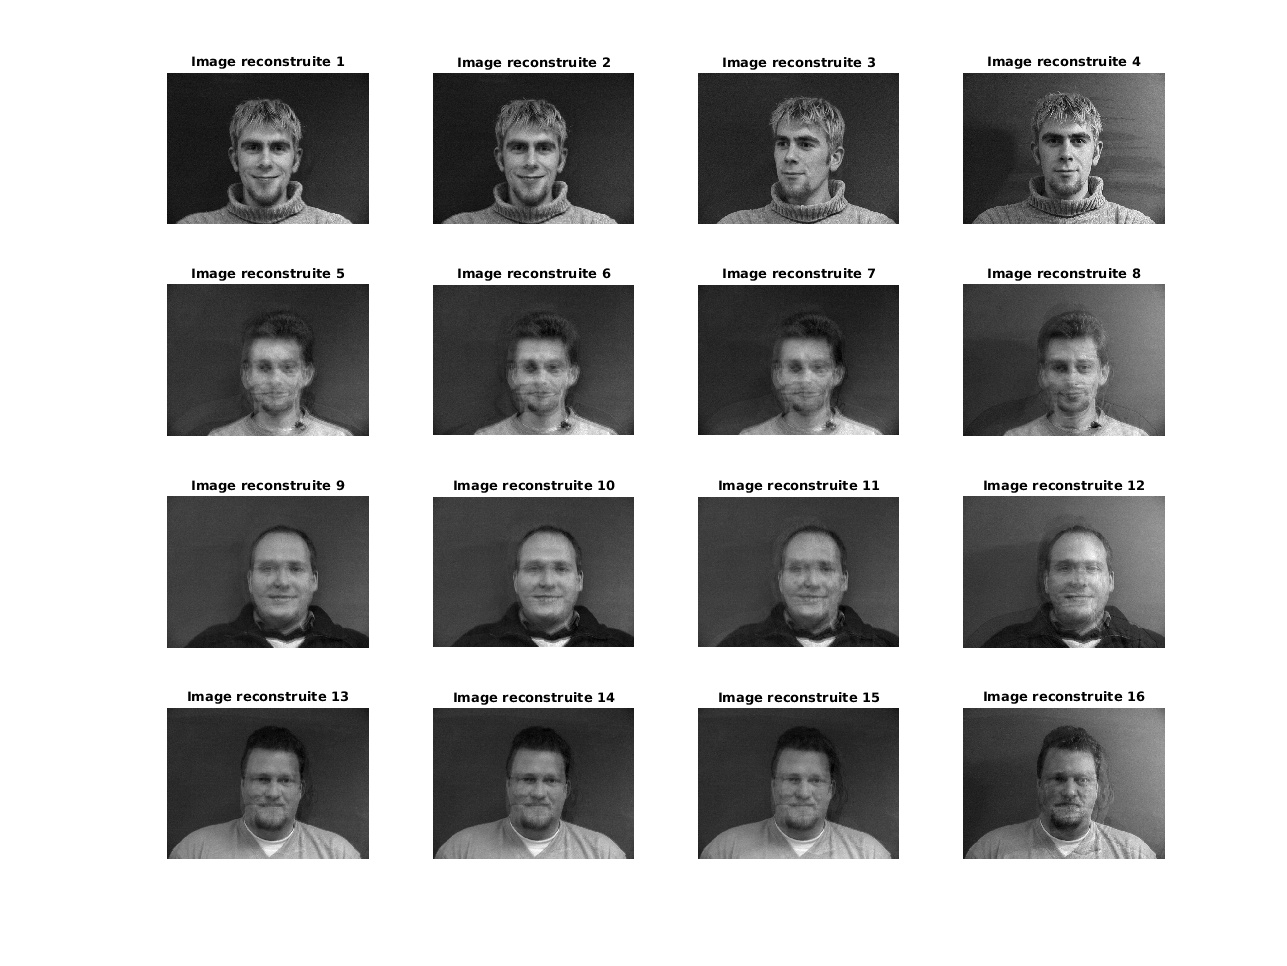
\includegraphics[width=0.9\linewidth]{images/2/2-2-res6.png}
        \caption{Projections des visages sur un sous espace composé des 6 eigenfaces principales}
        \label{proj_faces}
    \end{center}
\end{figure}
Ici on remarque que les images ne sont toute pas aussi bien conservées. En effet celles de l'individu 1 sont bien plus ressemblantes des images originales que celles des individus 2, 3, et 4 (ces dernières sont assez floues). Cela vient certainement du fait que les images de ce premier individu sont bien plus proches de l'individu moyen que les autres (un peu comme dans de cas de l'ACP d'une image dont le contraste est principalement dû à sa composante bleu, sa composante principale sera alors proche de sa composante bleu). De plus on observe que les projections des images de l'individu 4 se ressemble beaucoup : cette fois cela doit venir du fait que les différences entre les images de cet individu sont très faibles et donc leur informations doivent être contenues selon des composantes de l'ACP d'ordre bien plus élevés (et celles-ci ne sont pas ici conservées puisqu'on s'intéresse à tous les individus en même temps).

\paragraph{Comparaison selon la dimension du sous-espace}
Par la suite on calcul la moyenne de l'écart au carré des images à leurs projections dans des espaces issus de plus ou moins d'eigenfaces pour observer la différences de "respect de l'image originale" de ces différents espaces. Comme on pouvait s'y attendre, celle-ci diminue à mesure que l'on conserve d'avantage d'eigenfaces : cela n'est pas surprenant puisqu'on conserver alors des espaces plus grands qui vont permettre de mieux distinguer les images les unes des autres (voir figure~\ref{rmse}).
\begin{figure}[ht]
    \begin{center}
        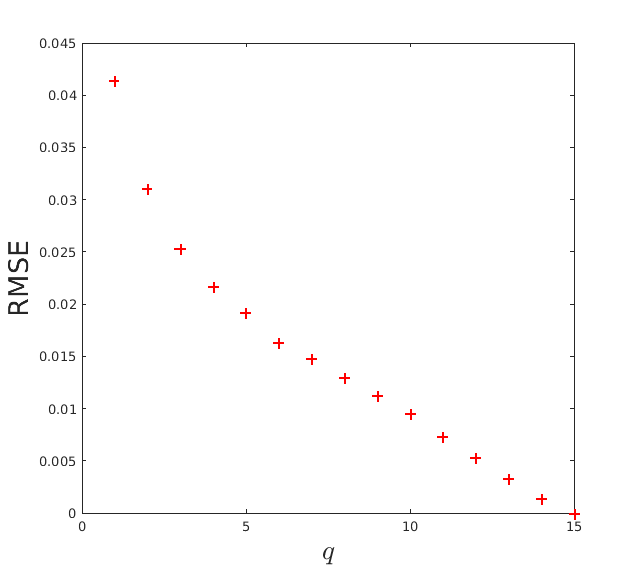
\includegraphics[width=0.6\linewidth]{images/2/2_2_rmse.png}
        \caption{RMSE en fonction du nombre de composantes principales conservées (sur 15)}
        \label{rmse}
    \end{center}
\end{figure}

\subsection{Exercice 3 - Restauration d'images dégradées}
Ici on décide de restaurer des images à partir de leur versions dégradées par une bande noire obstruant une partie plus ou moins grande de leur surface. Pour cela on projette donc l'image dégradée dans la base de issue de l'ACP puis on considère cette projection comme étant l'image non dégradée. Ainsi pour des bandes d'altération de tailles différentes on observe les résultats figure~\ref{reconstitution_bandes_noires}.
\begin{figure}[ht]
    \centering
    \begin{subfigure}[c]{0.7\linewidth}
    	\centering
    	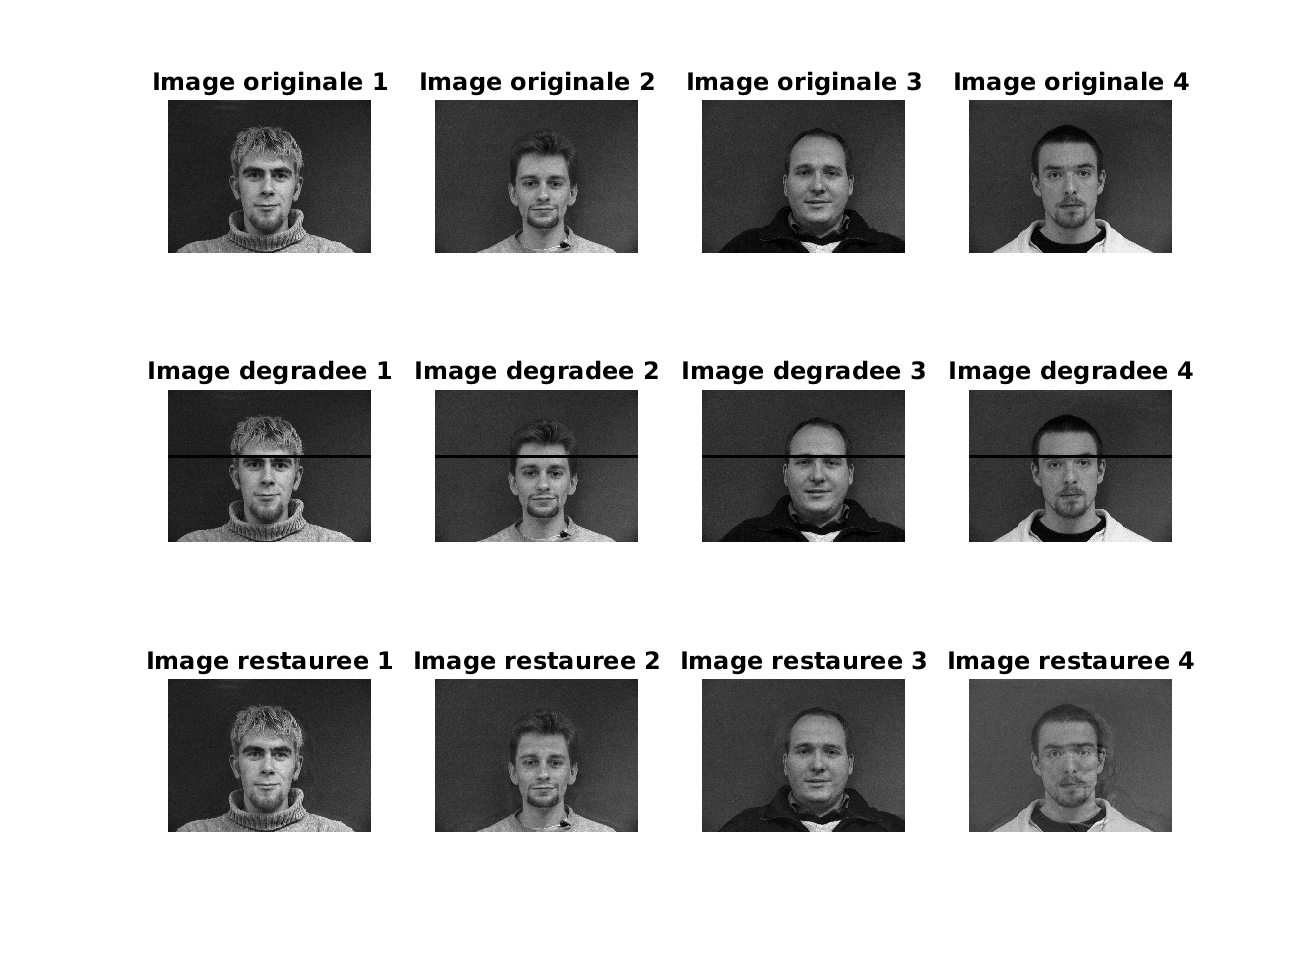
\includegraphics[width=\linewidth]{images/2/2-3-5.png}
    	\subcaption{Pour une bande noire de 5 pixels d'épaisseur}
    \end{subfigure}
    \begin{subfigure}[c]{0.7\linewidth}
    	\centering
    	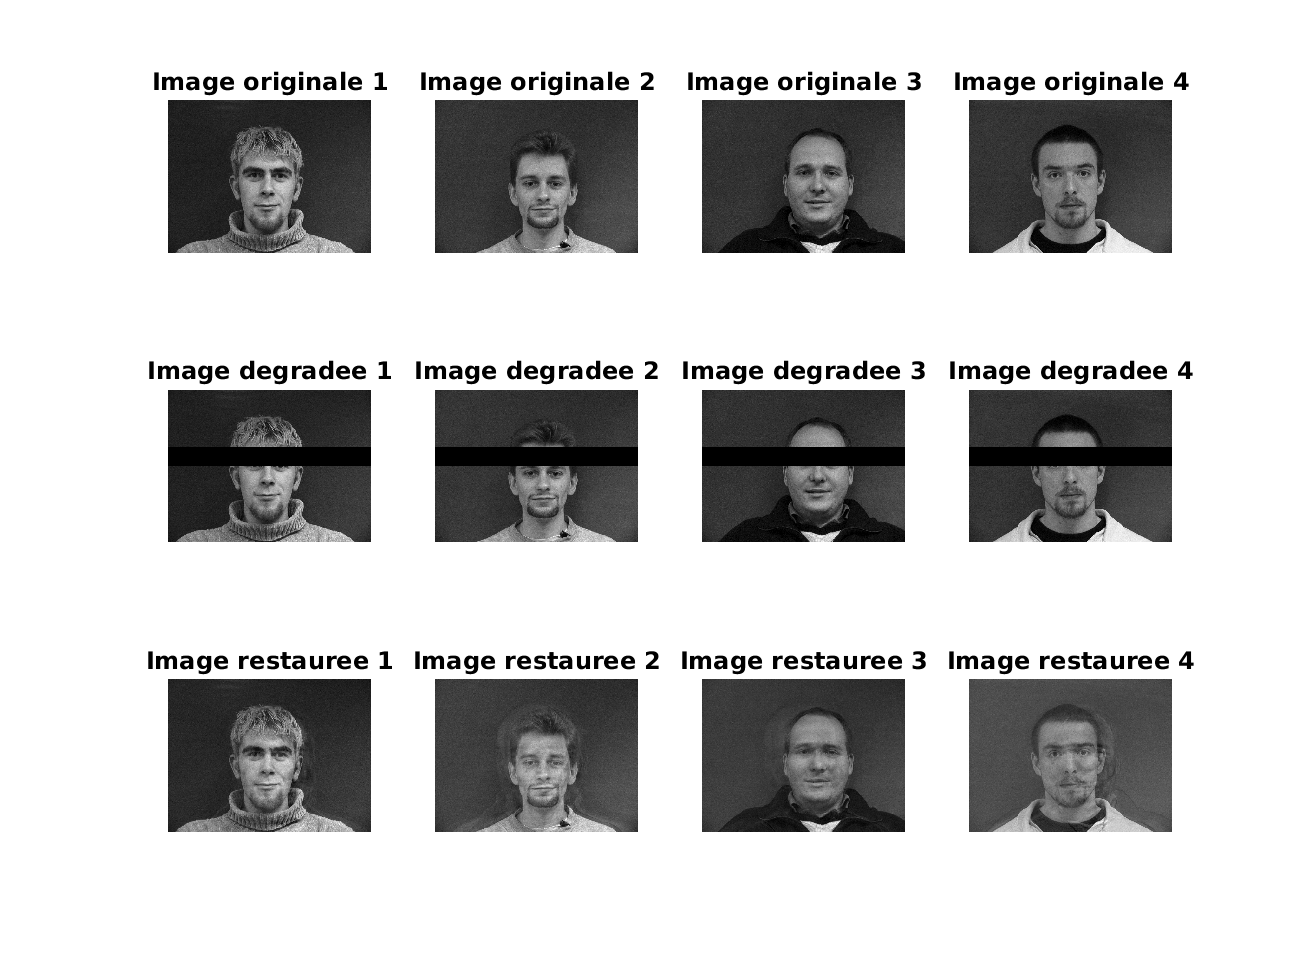
\includegraphics[width=\linewidth]{images/2/2-3-30.png}
    	\subcaption{Pour une bande noire de 30 pixels d'épaisseur}
    \end{subfigure}
    \caption{Restauration d'images dégradées par des bandes noires}
    \label{acp_gantrycrane}
\end{figure}

\section{TP3}
\subsection{Exercice 1}
Lorem upsum

\subsection{Exercice 2}
Lorem ypsum

\end{document}
